\chapter{シミュレーション結果}
\section{シミュレーション条件}
\label{sec:contdition}
シミュレーション条件として,基地局数2,基地局のアンテナ数128本,基地局当たりのユーザ数16人,送信フレーム長1000,パイロット信号の長さ300,通信路/データ推定器内における反復回数30回,両者の間の反復回数3回の場合を想定した.送信するデータは電力1のQPSK信号であり,送信するデータ構造は図\ref{fig:data_structure}に示す.
\begin{figure}[htbp]
  \begin{center}
    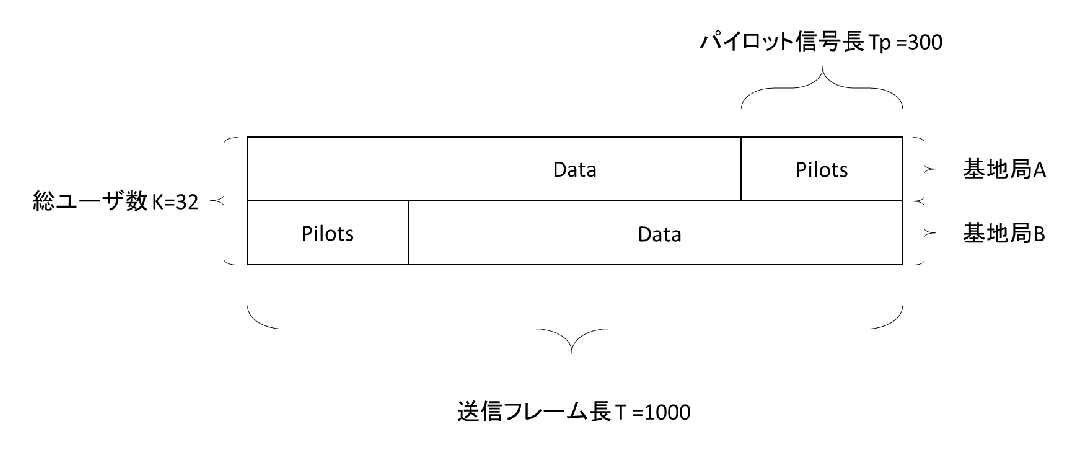
\includegraphics[clip,width=10.0cm]{./data_structure.eps}
    \caption{送信されるデータ構造}
    \label{fig:data_structure}
  \end{center}
\end{figure}

また,計算順序は以下のとおりである.
\begin{enumerate}
	\item 初期処理(通信路とデータの生成,メッセージの初期化)
	\item 通信路推定を30回繰り返す \label{estimate_h}
	\item データ推定を30回繰り返す  \label{estimate_x}
	\item \ref{estimate_h}.\ref{estimate_x}.を3回繰り返す
	\item 終了処理
\end{enumerate}
なお,以下に示す結果はすべて50回のアンサンブル平均で示す.
\section{通信路推定}
横軸に反復回数,縦軸に通信路推定の平均二乗誤差(MSE)をとり,SNRごとに出力したものを図\ref{fig:mse_h}に示す.反復回数30回ごとにデータ推定を行い,再び通信路推定を行ったときにMSEが減少していることが確認できる.また,SNR=10dBのときの時間シフト送信データフレームと,同期送信データフレームのMSEの比較した図を図\ref{fig:mse_h_comparison}に示す.一回目の通信路推定では,シフトフレームはMSE=0.126566に対し,同期フレームはMSE=0.095458であったが最終的にシフトフレームはMSE=0.025941,同期フレームはMSE=0.026116であり,反復を振り返すと,二つのMSEの差は小さくなった.
\begin{figure}[htbp]
  \begin{center}
    \includegraphics[clip,width=10.0cm]{./mse_h.eps}
    \caption{通信路推定の平均二乗誤差}
    \label{fig:mse_h}
  \end{center}
\end{figure}

\begin{figure}[htbp]
  \begin{center}
    \includegraphics[clip,width=10.0cm]{./mse_h_comparison.eps}
    \caption{通信路推定の平均二乗誤差 時間シフトフレームと同期フレームの比較(SNR=10dB)}
    \label{fig:mse_h_comparison}
  \end{center}
\end{figure}
\section{データ推定}
横軸に反復回数,縦軸にデータ推定のビット誤り率をとり,SNRごとに出力したものを図\ref{fig:bit_err}に示す.反復回数30回ごとに通信路推定を行い,再びデータ推定を行ったときにBERが減少していることが確認できる.また,SNR=10dBのときの時間シフト送信データフレームと,同期送信データフレームのBERを比較した図を図\ref{fig:bit_err_comparison}に示す.一回目のデータ推定では,シフトフレームBER=0.011804に対し,同期フレームはBER=0.002713であったが最終的にシフトフレームはBER=0.001163,同期フレームはBER=0.001170であり,反復を振り返すと,二つのBERの差は小さくなった.
また,横軸にSNR,縦軸にデータ推定のビット誤り率をとり出力したものを図\ref{fig:sn_bit_err}に示す.SNRの上昇に伴いBERも減少していくことが確認できた.
\begin{figure}[htbp]
  \begin{center}
    \includegraphics[clip,width=10.0cm]{./bit_err.eps}
    \caption{データ推定のBER}
    \label{fig:bit_err}
  \end{center}
\end{figure}
\begin{figure}[htbp]
  \begin{center}
    \includegraphics[clip,width=10.0cm]{bit_err_comparison.eps}
    \caption{データ推定のBER 時間シフトフレームと同期フレームの比較(SNR=10dB)}
    \label{fig:bit_err_comparison}
  \end{center}
\end{figure}
\begin{figure}[htbp]
  \begin{center}
    \includegraphics[clip,width=10.0cm]{./sn_bit_err.eps}
    \caption{データ推定のBER}
    \label{fig:sn_bit_err}
  \end{center}
\end{figure}